% !TeX root = induction-he.tex

\chapter{%
לא רק חשבון%
}\label{s.notjust}

כמעט תמיד מלמדים אינדוקציה בצורה של אינדוקציה מתמטית מעל למספרים השלמים החיוביים. אולם, השיטה מתאימה בכל מצב בו מבנים גדולים בנויים ממבנים קטנים יותר.
\textbf{אינדוקציה מעל מבנה}
נמצאת בשימוש נרחב במדעי המחשב, שם מבני נתונים מוגדרים בצורה רקורסיבית. בפרק זה נציג דוגמאות של השימוש באינדוקציה במבנים מתמטיים שהם לא מספרים שלמים: טריגונומטריה, פוליגונים, גרפים ועצים. נתחיל בדוגמה של אינדוקציה מעל מבנה.

\begin{definition}
\textbf{ביטוי}
)חשבוני( מורכב ממשתנים וקבועים ביחד עם הפעולות הבונות:
\begin{quote}
אם
$E_1, E_2$
הם ביטויים, אזי גם
$(E_1+E_2), (E_1-E_2), (E_1\times E_2), (E_1/E_2)$
הם ביטויים.%
\footnote{%
חוקים של קדימויות יכולים להקטין את מספר הסוגריים, כך שהמשמעות של
$a\times b + 2$
היא
$((a\times b)+c)$
ולא
$(a\times (b+c))$.
בדיון כאן נתעלם מקדימויות.}
\end{quote}
\end{definition}

\begin{exercise}\mbox{}\\
)א( מספר הסוגרים השמאליים בביטוי שווה למספר הסוגרים הימניים.\\
)ב( בכל מקום בביטוי, מספר הסוגרים השמאליים משמאל לנקודה גדול או שווה למספר הסוגרים הימניים משמאלה.
\end{exercise}

\textbf{דוגמה}
בביטוי
$(x+(y-23))$
קיימים שני סוגרים שמאליים ושני סוגרים ימניים. במקום המסומן על ידי
$|$
בביטוי
$(x+(y\,|-23))$,
קיימים שני סוגרים שמאליים משמאל לסימן
$|$
ואפס סוגרים ימניים.

\section{%
טריגונומטריה%
}

\begin{theorem}\label{t.cos}
לכל
$n\geq 1$, $\cos n\pi = (-1)^n$\,.
\end{theorem}

\textbf{הוכחה}
טענת הבסיס פשוטה להוכחה:
$\cos 1\pi = \cos \pi = -1 = (-1)^1$.
הנחת האינדוקציה היא
$\cos n\pi = (-1)^n$.
הצעד האינדוקטיבי הוא:
\[
\cos (n+1)\pi = \cos (n\pi + \pi) = \cos n\pi \cdot \cos \pi - \sin n\pi \cdot \sin \pi\,.
\]
מ-%
$\sin \pi = 0$
ו-%
$\cos \pi = -1$
מתקבל:
\[
\cos (n+1)\pi = \cos n\pi \cdot -1 \ih{} (-1)^n \cdot -1 = (-1)^{n+1}\,.
\]

\qedd{7}

כאשר הוכחנו משפטים באמצעות אינדוקציה מתמטית מעל למספרים השלמים, ביצעו חישובים חשבוניים ואלגבריים ללא הנמקה. כאן, השתמשנו ללא הנמקה מפורשת בנוסחה טריגונומטית עבור 
$\cos (\alpha+\beta)$.

\begin{exercise}
לכל
$n\geq 1$:
\[
\cos\theta \cdot \cos 2\theta \cdot \cos 4\theta \cdot \cdots \cdot \cos 2^{n-1}\theta = \frac{\sin 2^n\theta}{2^n \sin \theta}\,.
\]
\end{exercise}
\textbf{רמז} 
השתמש בנוסחה ל-%
$\sin 2\theta$.

\begin{exercise}
לכל
$n\geq 1$, $(\cos \theta + i\sin\theta)^n = \cos n\theta + i\sin n\theta$.
\end{exercise}

\section{%
גיאומטריה
}

במבט ראשון, קשה לראות איך אפשר להשתמש באינדוקציה בהוכחת משפטים בגיאומטריה. אולם, משפטים רבים מנוסחים בצורה: "לכל פוליגון עם
$n$
צלעות,
\ldots,"
ואינדוקציה מתאימה מאוד במקרים אלה.
\begin{theorem}\label{t.diag}
לכל פוליגון קמור עם
$n$
צלעות, מספר המשולשים הנוצרים מהאלכסונים
\textbf{שאינם נחתכים}
הוא
$n-2$.
\end{theorem}

\textbf{הוכחה}
במשולש אין אלכסונים, 
$n=3$
ויש משולש אחד:
$3-2=1$.
טענת בסיס טובה יותר היא עבור מרובע 
$n=4$.
קיים אלכסון אחד שאינו חותך אלכנסון אחר והוא מייצר
$4-2=2$
משולשים.

נקח פוליגון עם
$n+1$
צלעות ונצייר אלכסון אחד בין שני צמתים השכנים לצומת אחר. האלכסון ביחד עם הצלעות האחרים מהווים פוליגון עם
$n$
צלעות. לפי הנחת האינדוקציה, האלכסונים שאינם חותכים אחד את השני מייצרים 
$n-2$
משולשים. עם המשולש החדש, קיימים
$(n-2)+1=(n+1)-2$
משולשים.
\qed

\textbf{דוגמה}
תרשים~%
\ref{fig.diag}
מראה משושה 
$n=6$.
צייר את הקו
$AE$
המחלק את המשושה למשולש
$AEF$
ולמחומש
$ABCDE$.
צייר את האלכסונים שאינם נחתכים
$AC$
ו-
$AD$.
לפי הנחת האינדוקציה, מספר המשולשים במחומש הוא
$5-2=3$: $ABC$, $ACD$, $ADE$.
ביחד עם המשולש
$AEF$,
קיימים
$6-2=4$
משולשים.

\begin{figure}[t]
\begin{center}
\selectlanguage{english}
\begin{tikzpicture}
\node[name=hexagon, regular polygon, regular polygon sides=6, minimum size=4cm, draw] at (0,0) {};
\draw (hexagon.corner 2) -- (hexagon.corner 4);
\draw [dashed] (hexagon.corner 2) -- (hexagon.corner 5);
\draw [dashed] (hexagon.corner 2) -- (hexagon.corner 6);
\foreach \anchor/\placement/\name in {corner 1/above/$B$, corner 2/above/$A$, corner 3/left/$F$, corner 4/below/$E$, corner 5/below/$D$, corner 6/right/$C$}
\draw (hexagon.\anchor) node[\placement] {\name};
\end{tikzpicture}
\selectlanguage{hebrew}
\caption{
\R{אלכסונים שלא נחתכים}
}\label{fig.diag}
\end{center}
\end{figure}

\begin{exercise}\label{e.diag}
עבור פוליגון קמור עם
$n$
צלעות, מספר האלכסונים )כולל אלה שנחתכים( הוא
$\frac{1}{2}n(n-3)$.
\end{exercise}
\begin{exercise}
עבור פוליגון קמור עם
$n$
צלעות, סכום הזוויות הפנימיות הוא
$180(n-2)^{\circ}$.
\end{exercise}
\begin{exercise}
נתון קו באורך
$1$
ומספר שלם
$n\geq 1$,
בנה קו באורך
$\sqrt n$.
\end{exercise}
\textbf{רמז}
משפט פיתגורס.

\section{%
עצים%
}

\textbf{עץ בינרי}
הוא גרף עם צמתים וקשתות, כאשר יש צומת אחד הנקרא השורש ולכל צומת יש אפס, אחת או שתי קשתות היוצאות ממנו אל צמתים אחרים הנקראים בנים. אין מעגלים בעץ. צומת ללא בנים נקרא עלה וצומת שהוא לא עלה נקרא צומת פנימי. גובה עץ
$h$
הוא אורך המסלול הארוך ביותר בין השורש לבין עלה. עץ בינרי שכל העלים בו הם באותו גובה ושלכל הצמתים הפנימיים בו יש שני בנים נקרא
\textbf{עץ בינרי שלם}
)תרשים~%
\ref{fig.complete}(.

\begin{figure}[h]
\begin{center}
\selectlanguage{english}
\begin{tikzpicture}%
[scale=.9,dots/.style={fill, inner sep=0pt, minimum size=3pt, shape=circle},%
level 1/.style={sibling distance=2cm},%
level 2/.style={sibling distance=1.5cm}]

\node[dots] at (7.5,0) {}
child {
  node[dots] {} coordinate (L1)
  child { node[dots] {} coordinate (L2)}
  child { node[dots] {}}
}
child {
  node[dots] {}
  child { node[dots] {}}
  child { node[dots] {}}
};

\node[dots] at (3,0 |- L1) {}
child { node[dots] {}}
child { node[dots] {}};

\node[dots] at (0,0 |- L2) {};

\node at (0,-3.5) {(a)};
\node at (3,-3.5) {(b)};
\node at (7.5,-3.5) {(c)};
\end{tikzpicture}
\selectlanguage{hebrew}
\caption{%
עצים בינריים שלמים בגובה
$0$, $1$, $2$
}\label{fig.complete}
\end{center}
\end{figure}

\vspace*{-6ex}

\begin{theorem}
יהי 
$n_h$
מספר הצמתים בעץ בינרי שלם בגובה 
$h$.
אזי
$n_h = 2^{h+1}-1$.
\end{theorem}

\textbf{דוגמה} 
בתרשים~%
\ref{fig.complete}: \L{(a)} $n_0=2^1-1=1$,$\,$ \L{(b)} $n_1 = 2^2-1=3$,$\,$ \L{(c)} $n_2 = 2^3-1=7$.

\textbf{הוכחה} 
הוכחת טענת הבסיס פשוטה: עלה הוא עץ בגובה אפס ו-%
$1 = 2^{0+1}-1=1$.
הנחת האינדוקציה היא שמספר הצמתים בתת-עץ השמאלי
$n_l$
ומספר הצמתים בתת-עץ הימני
$n_r$,
שניהם בגובה
$h$,
ניתנים על יד הנוסחה
$n_l=n_r=2^{h+1}-1$.
כדי להוכיח את הצעד האינדוקטיבי, נשים לב שעץ בגובה 
$h+1$
בנוי משני תת-עצים בגובה
$h$,
ביחד עם צומת אחד נוסף שהוא השורש החדש. לכן:
\[
n_{h+1} = n_l + n_r + 1 \ih{} (2^{h+1}-1) + (2^{h+1}-1) + 1 = 2\cdot 2^{h+1} -2 +1= 2^{(h+1)+1} - 1\,.
\]

\qedd{5}

למרות שהאינדוקציה היא אינדוקציה מתמטית על גובה העץ, העץ עצמו בנוי משני תת-עצים שלכל אחד מהם יש מעט פחות ממחצית הצמתים. בתרגיל הבא צורת האינדוקציה הזאת תתבהר.
\begin{exercise}
יהי
$n_h$
מספר הצמתים בעץ בינרי )לא בהכרח שלם( בגובה
$h$.
אזי
$n_h\leq 2^{h+1}-1$.
\end{exercise}

\textbf{דוגמה} 
תרשים~%
\ref{fig.incomplete}
מראה עץ בינרי בגובה
$2$
עם
$5 \leq 2^3-1=7$
צמתים.

\begin{figure}[t]
\begin{center}
\selectlanguage{english}
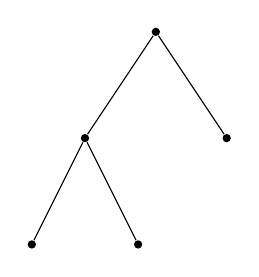
\begin{tikzpicture}%
[scale=.9,dots/.style={fill, inner sep=0pt, minimum size=3pt, shape=circle},%
level 1/.style={sibling distance=2cm},%
level 2/.style={sibling distance=1.5cm}]
\node[dots] at (0,0) {}
child {
  node[dots] {}
  child { node[dots] {}}
  child { node[dots] {}}
}
child {
  node[dots] {}
};
\end{tikzpicture}
\selectlanguage{hebrew}
\caption{%
עץ בינרי לא שלם בגובה
$2$
עם
$5$
צמתים
}\label{fig.incomplete}
\end{center}
\end{figure}

\section{%
גרפים%
}

גרף הוא מבנה כללי המורכב מצמתים וקשתות בין הצמתים. אם הקשתות מרכיבות מסלול סגור, הן תוחמות שטח. אנחנו גם סופרים כשטח את כל המישור מחוץ לגרף. התרשים להלן מראה גרף עם
$7$
צמתים,
$8$
קשתות, ו-%
$3$
שטחים, כאשר 
$s_3$
מופיע מספר פעמים כדי להדגיש את השטח של המישור מחוץ לגרף.

%\begin{figure}[hbt]
\begin{center}
\selectlanguage{english}
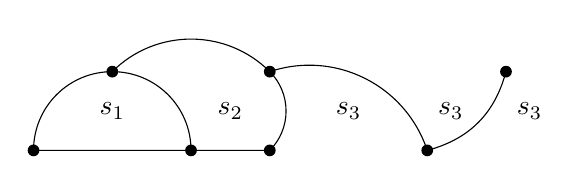
\begin{tikzpicture}
\draw (0,0) to [bend left=45] (1,1) to [bend left=45] (3,1) to [bend left=45] (3,0) to cycle;
\draw (1,1) to [bend left=45] (2,0);
\draw (3,1) to [bend left=45] (5,0) to [bend right=30] (6,1);
\foreach \x in {(0,0),(1,1),(2,0),(3,0),(3,1),(5,0),(6,1)}
  \node[shape=circle,fill,inner sep=1.5pt] at \x {};
\foreach \x/\i in {1/$s_1$,2.5/$s_2$,4/$s_3$,5.3/$s_3$,6.3/$s_3$}
  \node at (\x,0.5) {\i};
\end{tikzpicture}
%\caption{A graph with $7$ nodes, $8$ edges and $3$ surfaces}\label{fig.euler}
\end{center}
%\end{figure}

\begin{exercise} \textbf{\L{(Euler)}}
עבור גרף עם
$n$
צמתים,
$e$
קשתות ו-%
$s$
שטחים, מתקיים 
$s+n=e+2$.
\end{exercise}
\textbf{דוגמה}
בתרשים, 
$3+7=8+2$.

\textbf{רמז}
הוכח באמצעות אינדוקציה על מספר הקשתות בגרף. יש שני צעדים אינדוקטיביים, תלוי אם הקשת היא חלק ממסלול סוגר או לא.

%%%%%%%%%%%%%%%%%%%%%%%%%%%%%%%%%%%%%%%%%%%%%%%%%%%%%%%%%%%%%%%%%%%
